%% FullCourse_10Lecs -- Lecture 6, Topic 6.2b: Global Solution via DNN
%% Source: ./archive_pre_split/Lec06_HA_Models.tex (section 5)
%% Sub-split: original T2 (sections 3-5) exceeded 30-page ceiling at 33 pages.
%% Split into T2a (sections 3-4) and T2b (section 5).

%% Shared preamble for the FullCourse_10Lecs topic decks.
%%
%% Each topic .tex \input's this file, then defines its own \title, \date
%% override (if any), \graphicspath, and \begin{document}.
%%
%% Reconstructed verbatim from the inlined copy preserved in
%% Lec10_Case_Studies/Lec10_T8_Case6_DeepRamsey.tex (lines 23-190), which is
%% explicitly annotated there as "from ../shared_preamble.tex, copied verbatim".
%% Base preamble matches MiniCourse_8hr/Slides/shared_preamble.tex; this version
%% additionally provides \sectiondivider, the conceptbox/cautionbox/examplebox/
%% takeawaybox tcolorboxes, and \compacttables used across the split decks.

\documentclass[10pt,english,aspectratio=169]{beamer}

\usepackage{ae,aecompl}
\usepackage[T1]{fontenc}
\usepackage{textcomp}
\usepackage[utf8]{inputenc}
\usepackage{babel}
\usepackage{datetime2}

\setcounter{secnumdepth}{3}
\setcounter{tocdepth}{3}

\usepackage{amsmath, amssymb, amsthm, graphicx}
\usepackage{booktabs, multirow}
\usepackage{tikz}
\usepackage{pgfplots}
\pgfplotsset{compat=1.16}
\usepackage[most]{tcolorbox}
\tcbuselibrary{skins, breakable, theorems}
\usepackage{listings}
\usepackage{xcolor}

\lstset{
  basicstyle=\ttfamily\small,
  keywordstyle=\color{blue!80!black}\bfseries,
  commentstyle=\color{green!50!black}\itshape,
  stringstyle=\color{orange!80!black},
  backgroundcolor=\color{gray!8},
  frame=single,
  rulecolor=\color{gray!40},
  breaklines=true,
  showstringspaces=false,
  numbers=none,
}

\lstdefinestyle{pythonstyle}{
    language=Python,
    basicstyle=\ttfamily\footnotesize,
    keywordstyle=\color{blue!80!black}\bfseries,
    commentstyle=\color{green!50!black}\itshape,
    stringstyle=\color{orange!80!black},
    frame=single,
    breaklines=true,
    showstringspaces=false,
    numbers=left,
    numbersep=5pt,
    numberstyle=\tiny\color{gray},
    backgroundcolor=\color{gray!8},
    rulecolor=\color{gray!40}
}

\ifx\hypersetup\undefined
  \AtBeginDocument{%
    \hypersetup{bookmarks=false,breaklinks=true,pdfborder={0 0 0},colorlinks=true,
      linkcolor=DarkText,urlcolor=RedTitle}%
  }
\else
  \hypersetup{bookmarks=false,breaklinks=true,pdfborder={0 0 0},colorlinks=true,
    linkcolor=DarkText,urlcolor=RedTitle}%
\fi

\makeatletter
\newcommand\makebeamertitle{%
  \begin{frame}[plain]
    \vspace*{1.0cm}
    \centering
    {\usebeamerfont{title}\usebeamercolor[fg]{title}\inserttitle\par}
    \vspace{1.0cm}
    {\usebeamerfont{author}\usebeamercolor[fg]{author}\insertauthor\par}
    \vspace{0.2cm}
    {\usebeamerfont{date}\usebeamercolor[fg]{date}\insertdate\par}
  \end{frame}}%
\AtBeginDocument{%
  \let\origtableofcontents=\tableofcontents
  \def\tableofcontents{\@ifnextchar[{\origtableofcontents}{\gobbletableofcontents}}
  \def\gobbletableofcontents#1{\origtableofcontents}%
}

\usetheme{metropolis}
\usefonttheme{professionalfonts}

\definecolor{LightGray}{RGB}{230,230,230}
\definecolor{RedTitle}{RGB}{0,0,200}
\definecolor{VeryLightGray}{RGB}{245,245,245}
\definecolor{DarkText}{RGB}{0,0,0}

\setbeamercolor{background canvas}{bg=white}
\setbeamercolor{title}{fg=RedTitle}
\setbeamercolor{author}{fg=DarkText}
\setbeamercolor{date}{fg=DarkText}
\setbeamercolor{frametitle}{bg=VeryLightGray,fg=DarkText}
\setbeamercolor{normal text}{fg=DarkText}
\setbeamerfont{title}{size=\large}

\setbeamersize{text margin left=5mm, text margin right=5mm}
\addtobeamertemplate{frametitle}{}{\vspace{-0.5em}}
\newcommand{\reducevspace}{\vspace{-0.5cm}}

% Shared section divider and box styles for split topic decks.
\newcommand{\sectiondivider}[2]{%
\begin{frame}[plain,noframenumbering]
\begin{center}
\vfill
{\Large\textbf{#1}\par}
\vspace{0.35cm}
{\normalsize #2\par}
\vfill
\end{center}
\end{frame}
}

\newtcolorbox{conceptbox}[1][]{
  colback=blue!3,
  colframe=RedTitle!55,
  boxrule=0.35mm,
  arc=1mm,
  left=2mm,
  right=2mm,
  top=1mm,
  bottom=1mm,
  #1
}
\newtcolorbox{cautionbox}[1][]{
  colback=red!3,
  colframe=red!50!black,
  boxrule=0.35mm,
  arc=1mm,
  left=2mm,
  right=2mm,
  top=1mm,
  bottom=1mm,
  #1
}
\newtcolorbox{examplebox}[1][]{
  colback=green!3,
  colframe=green!45!black,
  boxrule=0.35mm,
  arc=1mm,
  left=2mm,
  right=2mm,
  top=1mm,
  bottom=1mm,
  #1
}
\newtcolorbox{takeawaybox}[1][]{
  colback=VeryLightGray,
  colframe=RedTitle!55,
  boxrule=0.35mm,
  arc=1mm,
  left=2mm,
  right=2mm,
  top=1mm,
  bottom=1mm,
  #1
}
\newcommand{\compacttables}{\renewcommand{\arraystretch}{1.15}}

\setbeamertemplate{navigation symbols}{}
\setbeamertemplate{footline}{%
  \hfill%
  \usebeamercolor[fg]{page number in head/foot}%
  \usebeamerfont{page number in head/foot}%
  \insertframenumber\,/\,\inserttotalframenumber\kern1em\vskip2pt%
}

\makeatother

\author{Zhigang Feng}
% "date with time": compile timestamp so each build is identifiable.
\date{\today\ \DTMcurrenttime}


\graphicspath{{./pic/}{../../MiniCourse_8hr/Slides/Module2_DL_RL_Macro/pic/}{../}}

\title[AI for Econ Research]{AI for Economic Research: Dynamic Models, Language, and Agents\\
Lecture 6.2b: Global Solution via Deep Neural Networks}

\begin{document}

\makebeamertitle

%=============================================================================
\begin{frame}{Topic 6.2b Agenda}
\begin{enumerate}
  \item \textbf{Global Solution via DNN} --- full distribution as state, value/policy networks
\end{enumerate}
\medskip
\textit{Arc: T1 Aiyagari + computation $\to$ T2a Why ML / Euler $\to$ \textbf{T2b Global DNN} $\to$ T3 KS / DeepHAM $\to$ T4 DEQN / OLG $\to$ T5 MFG $\to$ Lab06}
\end{frame}

%=============================================================================
\section{Global Solution via DNN}

\begin{frame}{Why (deep) RL helps}
Three reasons NN-based methods outperform grid methods on HA models:
\medskip
\begin{enumerate}
\item \textbf{Flexible function approximation.}\\
No structured Cartesian grid; networks handle high-dimensional inputs gracefully.
\medskip
\item \textbf{Sampling-based training.}\\
RL methods were designed for unknown environments; here we re-use the data-generation tools (rollouts, replay, importance sampling) even though our model is known. This avoids constructing exhaustive grids or closed-form distribution evolution.
\medskip
\item \textbf{Hardware acceleration.}\\
Forward/backward passes through neural networks are highly parallel matrix operations that GPUs and TPUs execute efficiently. Grid VFI is much harder to parallelise.
\end{enumerate}
\end{frame}

\begin{frame}{Global solution: full distribution as part of the state}
\begin{itemize}
\item In Aiyagari we exploited \emph{stationarity}: the distribution $\lambda$ was a fixed object and dropped out of the household state.
\medskip
\item Once we add aggregate shocks, $\lambda_t$ becomes part of the dynamic state. The household problem is
\[
V(a, z, \lambda) = \max_{c,a'}\!\left\{u(c) + \beta\,\mathbb{E}\!\left[V(a', z', \lambda')\,|\,z\right]\right\}.
\]
\item The law of motion for $\lambda$ is
\[
\lambda' \;=\; G(\lambda, Z, Z'),
\]
itself induced by the policy $a'(\cdot, \cdot, \lambda)$ and the shock kernel.
\item $\lambda$ is an infinite-dimensional object --- this is the heart of the curse of dimensionality in HA models with aggregate shocks.
\end{itemize}
\end{frame}

\begin{frame}{Household problem with an evolving distribution}
At the individual level, with state $(a,z,\lambda)$:
\[
V(a,z,\lambda) \;=\; \max_{a'}\!\left\{u\!\big((1+r(\lambda))a + w(\lambda)z - a'\big) + \beta\,\mathbb{E}\!\left[V(a',z',\lambda')\,|\,z\right]\right\}
\]
with $\lambda' = G(\lambda, Z, Z')$.
\medskip
\begin{itemize}
\item Two challenges:
  \begin{enumerate}
  \item How to represent $\lambda$ compactly enough that a NN can take it as input.
  \item How to evolve $\lambda$ forward without simulating $\sim 10^6$ agents.
  \end{enumerate}
\medskip
\item Three families of solutions:
  \begin{itemize}
  \item \emph{Moment approximations} (Krusell--Smith): summarise $\lambda$ by a few moments.
  \item \emph{Generalised moments} (DeepHAM): let the network learn the right summary statistics.
  \item \emph{Histogram transport} (DEQN): keep the full discretised distribution.
  \end{itemize}
\end{itemize}
\end{frame}

\begin{frame}{Approximating the distribution as a NN input}
\begin{center}
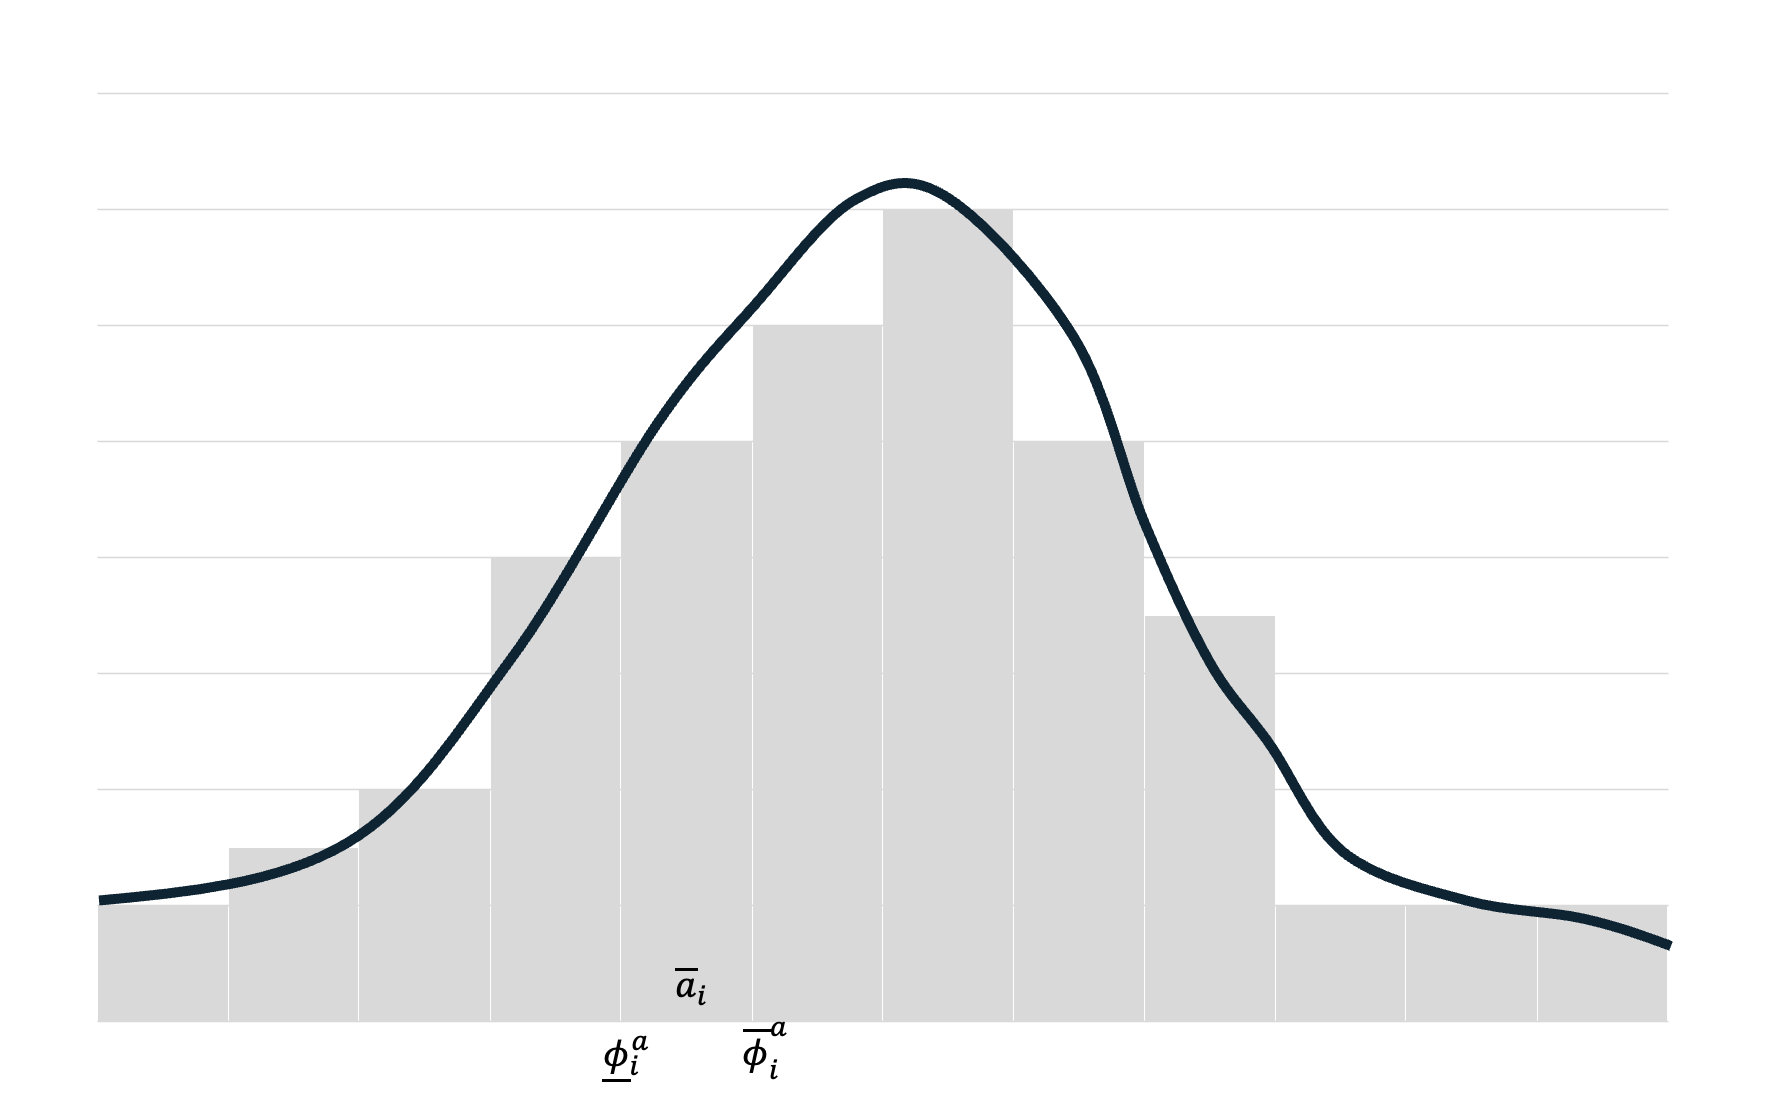
\includegraphics[width=0.55\textwidth]{app_dist}
\end{center}
\vspace{-0.5em}
\begin{itemize}
\item One option: discretise $\lambda$ on a fixed grid, feed the histogram heights to the NN.
\item Another: pass a finite vector of moments (means, variances, percentiles).
\item DeepHAM: \emph{learn} basis functions $Q_1,\ldots,Q_J$ and feed $\frac{1}{N}\sum_i Q_j(a_i)$ as moments.
\end{itemize}
\end{frame}

\begin{frame}{DNN representation of $V$ and the policy}
Parameterise
\[
V(S;\theta^V), \qquad c(S;\theta^c), \qquad S = (a, z, \lambda).
\]
\medskip
\begin{itemize}
\item Each network is a multilayer perceptron with parameters $\theta = (\text{weights}, \text{biases})$.
\item Inputs: individual state $(a,z)$ + summary of $\lambda$ (moments or generalised moments).
\item Outputs: scalar $V$, scalar consumption (or savings rate).
\medskip
\item Activations: ReLU, GELU, Mish --- all popular for HA-style problems.
\item Initialisation: Xavier/Glorot or Kaiming, depending on the activation.
\end{itemize}
\end{frame}

\begin{frame}{Update value function via simulation + supervised learning}
Given current policy $f_\sigma^{(n)}$, generate $N_V$ initial states $\{S_{i,0}\}_{i=1}^{N_V}$ and simulate $T_V$ periods forward. Compute the empirical (truncated) discounted utility:
\[
\hat V(S_{i,0}) \;=\; \sum_{t=0}^{T_V-1} \beta^t \, u(c_{i,t}).
\]
\medskip
Train the value network by supervised regression:
\[
\theta^{V,(n+1)} \;\in\; \arg\min_{\theta^V}\;
\sum_{i=1}^{N_V} \big(V(S_{i,0};\theta^V) - \hat V(S_{i,0})\big)^2.
\]
\medskip
\begin{itemize}
\item This is sometimes called \emph{Monte Carlo value estimation}.
\item Larger $T_V$ reduces bias but increases variance and cost.
\end{itemize}
\end{frame}

\begin{frame}{Update policy with terminal value function}
Given the just-updated value network $V(\cdot;\theta^{V,(n+1)})$, choose policy parameters to maximise the truncated objective with terminal value:
\[
\theta^{c,(n+1)} \;\in\; \arg\max_{\theta^c}\;
\mathbb{E}\!\left[\sum_{t=0}^{T_g-1}\beta^t u(c_{i,t}) + \beta^{T_g}\, V(S_{i,T_g};\theta^{V,(n+1)})\right]
\]
subject to the budget constraint
\[
c_{i,t} = (1+r(\lambda_t))\,a_{i,t} + w(\lambda_t)\,z_{i,t} - a'_{i,t},
\quad a'_{i,t} = c(S_{i,t};\theta^c).
\]
\medskip
This is a long-horizon \emph{differentiable rollout}: gradients propagate through the simulated path.
\end{frame}

\begin{frame}{Transition function $G$ as a matrix}
On a discretised asset grid $\{a_1,\ldots,a_{N_a}\}$, the policy $a'(\cdot)$ together with the shock kernel induces a Markov matrix
\[
\hat G_{i,j} \;=\; \Pr\!\big(a' \in \phi_j^a \,\big|\, a \in \phi_i^a\big),
\]
where $\phi_j^a$ are the discretisation cells.
\medskip
\begin{itemize}
\item $\hat G$ has $O(N_a^2)$ entries; sparse if the policy moves between adjacent cells.
\item Updating $\lambda$ one period: $\lambda^{(t+1)} = \hat G^\top \lambda^{(t)}$.
\item The same matrix is used in classical Aiyagari computation; here we re-use it inside the differentiable training loop.
\end{itemize}
\end{frame}

\begin{frame}{Conditional and unconditional transition kernels}
\textbf{Unconditional:}
\[
\lambda'(z' \in Z',\, a' \in A')
\;=\;
\int_{Z\times A} \mathbb{1}\!\big\{a'(a,z,\lambda)\in A',\; z'(a,z,\lambda)\in Z'\big\}\, d\lambda(z,a).
\]
\medskip
\textbf{Conditional (given current $(a,z)$):}
\[
\lambda'(z' \in Z',\, a' \in A' \mid z\in Z, a\in A)
=
\int_{Z\times A}\!\!\mathbb{1}\!\{\cdots\}\, d\lambda(z,a) \;/\; \lambda(Z\times A).
\]
\medskip
\begin{itemize}
\item Both kernels live in the Wasserstein space of probability measures on $S$.
\item The induced \emph{stochastic process on distributions} is the analytical object that DeepHAM and DEQN approximate by neural networks.
\end{itemize}
\end{frame}

\begin{frame}{Discretised transition: i.i.d.\ shocks, monotone policy}
When $z$ is i.i.d.\ and the policy $a'(a,z)$ is monotone in $a$ for each $z$, we can solve for transition cell boundaries explicitly:
\[
\hat G^{\lambda,\eta_x}_{i,j}
\;=\; \Pr\!\big(\phi_j^a \ni a_+ \leq \bar\phi_j^a \,\big|\, a \in \phi_i^a\big)
\;=\; F_z(\bar z_{i,j}) - F_z(\underline z_{i,j}),
\]
where $(\underline z_{i,j}, \bar z_{i,j})$ are the income shock thresholds that map $\phi_i^a$ to the boundaries of $\phi_j^a$ under the policy.
\medskip
\begin{itemize}
\item Closed-form bin probabilities $\Rightarrow$ no Monte Carlo noise in the $\lambda$-update.
\item Differentiability is delicate: the indicator functions inside the kernel are non-smooth, and need to be replaced by smooth approximations (e.g.\ sigmoids with sharp slopes) for gradient propagation.
\end{itemize}
\medskip
\emph{Next (T3):} Krusell--Smith with aggregate uncertainty, and DeepHAM as the deep-learning solution.
\end{frame}

\end{document}
